\chapter{Design}
\label{sec:design}

% Ist das zentrale Kapitel der Arbeit. Hier werden das Ziel sowie die
% eigenen Ideen, Wertungen, Entwurfsentscheidungen vorgebracht. Es kann
% sich lohnen, verschiedene Möglichkeiten durchzuspielen und dann
% explizit zu begründen, warum man sich für eine bestimmte entschieden
% hat. Dieses Kapitel sollte - zumindest in Stichworten - schon bei den
% ersten Festlegungen eines Entwurfs skizziert werden.
% Es wird sich aber in einer normal verlaufenden
% Arbeit dauernd etwas daran ändern. Das Kapitel darf nicht zu
% detailliert werden, sonst langweilt sich der Leser. Es ist sehr
% wichtig, das richtige Abstraktionsniveau zu finden. Beim Verfassen
% sollte man auf die Wiederverwendbarkeit des Textes achten.

% Plant man eine Veröffentlichung aus der Arbeit zu machen, können von
% diesem Kapitel Teile genommen werden. Das Kapitel wird in der Regel
% wohl mindestens 8 Seiten haben, mehr als 20 können ein Hinweis darauf
% sein, daß das Abstraktionsniveau verfehlt wurde.

% Die Lösung kurz vorstellen. also du hast dich für die lösung mit dem dc network entschieden und das wurde bisher noch nicht vorgeschlagen in der wissenschaft. Dann sagen bevor du das prinzip vorstellt werden erstmal alle Teilnehmer, die in dem System vorkommen, vorgestellt. dazu auch das bild aus der technischen richtlinie benutzen, wo smartmeter und smart meter admin. welche netzwerke also han etc...
%Dann sagen, dass du erstmal auf das angreifermodell eingehst und dann dc netz erklären und dann die lösung vorschlagen.
%die lösung wurde noch nicht diskutiert, weil in der wissenschaft immer davon ausgegangen wurde, dass smart meter nicht sicher sind,wir gehen davon aus, dass ein smart meter vertraut werden kann und das man deshalb auch nicht auf das billing eingehen muss, weil das smart meter korrekt arbeitet und das billing deshalb trivial ist. der stromanbieter kann auch prüfen  bzw. die logeinträge sind fälschungssicher.

This chapter outlines the conceptual solution of this thesis to achieve privacy-preserving smart meters. The proposed protocol can be categorized as aggregation without a trusted third party. Before discussing the conceptual solution, the technical guideline from the BSI will be explained. The BSI is the cyber-security authority of the German government and is responsible for critical infrastructures such as smart grids in Germany.  The technical guideline TR-03109 resolves all security standards and security concepts that must be met by all power grid providers in Germany. Therefore, the technical guideline gives a good overview of the actual structure of the German power grid. After getting an overview of the power grid and its participants, an attacker model will be designed. The attacker model will introduce all necessary participants, what their motives are and what malicious motives they might pursue. Finally, the security protocol will be presented. It will be shown how the protocol can be integrated into the technical policy and how different potentially malicious participants are handled.
\section{A Privacy-Preserving Aggregation Scheme Using DC-Nets}
In [Cha3-85, Cha8-85, Chau-88], David Chaum proposes a protocol which he calls DC network. The DC network offers the possibility to achieve both sender anonymity and receiver anonymity in communication networks. The operation of the DC network is explained in the following.
\subsection{DC Networks}
The DC network uses the property that any finite alphabet can be numerated( e.g a=0, b=1 etc). If an numerated alphabet from 0 is given, then this alphabet forms an abelian group (modulo alphabet size). Because of the abelian group, simple mathematical operations like addition can be performed on the numerated letters in the alphabet.
In addition, a DC network assumes that messages are always sent that are of equal length. A participant in a DC network uses one or more keys with which it superposes the messages and one generated key is then communicated to exactly one participant. 
More precisely, each participant adds locally all key characters it generates. Then, the received keys from other participants are locally subtracted and finally, all meaningful characters (the message) that should be sent are added (modulo alphabet size). The result of the operation is distributed in the communication network and is called local superposition. 
The distributed superpositions are added together globally and the result is transmitted back to all participants. Thereby only the meaningful messages remain. If a participant does not want to send a meaningful message, the participant sends an empty message. The message consists only of zeros and is superposed with the key. The empty message reflects the neutral element in this structure. If all participants have sent only empty messages, the global result is a message only containing 0. If one of all participants have sent a meaningful message, the global superposition is the message. If more than one participant sent a meaningful message, then the result is the overlay of all sent messages and a single message from the overlay cannot be recovered. In the last case one speaks also of a collision. In order to solve this problem, the collision resolution algorithm with averaging can be used in a DC network. 
Exchanging keys to calculate the local sum can be very tedious. In addition, a different key must be exchanged for each message round. Otherwise it would be very easy to calculate the key from previously sent empty messages. Therefore, so-called pseudo-random number generators are commonly used. The participants share the initial values of the pseudo-random number generators with each other when they join the DC network. This can be done in the same way as the exchange of keys (e.g. a cryptographic key exchange procedure). Due to the deterministic property of PRNGs, the same sequence of numbers is always generated from an initial value. This in turn means that the initial value must remain secret and must not be revealed to any other participant, since otherwise the secret keys can be found out from the initial value. The consequence would be the loss of anonymity. The security of the DC network depends largely on how secure the PRNGs are. Therefore, the PRNGs that are used must be cryptographically secure.\\
\begin{figure}[tbp]
  \centering
  \includegraphics[scale=1]{images/Schlüsselgraph.png}
  \caption[Short description]{An example of a NILM analysis.}
  \label{fig:Appliance_Model}
\end{figure}
The principle of the DC network is illustrated graphically in figure 3.3 using a simple example. Figure 3.3 is also called the key graph of a DC network and shows 4 participants in a DC network that are connected to each other along a communication link. The outer participants have only one partner, the inner participants are connected to 2 partners. Each participant now exchanges keys with its direct partners. The outer partners need to exchange only one key and the inner ones exchange keys with two direct partners.
The mathematical operation indicates whether the participant adds or subtracts the exchanged key with the partner. In the example given in the figure, the user Petra would subtract the exchanged key with Rüdiger from the message and would have formed her local superposition. Rudiger would have to add the exchanged key with Petra to his message. He would also have to subtract the key he exchanged with Sabine from the result to calculate his local superposition. 

%peusodzufallsgeneratoren
\subsection{DC Network Protocol in a German Smart Grid}
The DC network is a scheme that can be used to achieve sender anonymity and receiver anonymity. Considering the use case of the thesis, the receiver anonymity does not have to be implemented. The aim is to anonymize the electricity consumption and send it to the electricity provider. In this case, the electricity provider is a public recipient and known to all participants. Therefore, the identity of the electricity provider does not need to be protected. Unlike in a normal DC network, in the proposed solution the participants do not want to communicate with each other, they only want to send their electricity consumption to the electricity provider. Therefore, the global superposition do not have to be distributed in the network but only calculated at the electricity provider. The only exception is when joining the DC network, there the customers have to perform a key exchange once to configure the initial value for the PRNG as explained in 3.3.2. The electricity supplier is generally regarded as an honest-but-curious adversary. However, in the proposed protocol, the electricity provider partly performs administrative tasks for the dc network. For this reason, an additional aim is to ensure that even stronger attacks can be prevented if the electricity provider takes on the role of the much more dangerous malicious adversary. \\
\\
\textbf{Protocol Header}
\\
\\\begin{figure}[tbp]
  \centering
  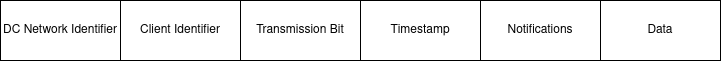
\includegraphics[width=1\textwidth]{images/Header.png}
  \caption[Short description]{An example of a NILM analysis.}
  \label{fig:Appliance_Model}
\end{figure}In the network protocol messages are sent which are structured in frames. The structure is shown in the figure 3.4. Each frame consists of a small header and the data part in which usually the local superposition is transfered. The purpose of each field is described further below.\\
As first field there is a Protocol Identifier field. The purpose of the Protocol Identifier field is to ensure that the application of the DC net protocol is recognized by all participants and that the SMGWs as well as the electricity provider can react correctly to the frames. This is followed by the DC Network Identifier field.%muss ich das hinschreiben?
The DC network identifier field offers the electricity provider the possibility to operate several DC networks in different regions and to distinguish DC networks. In addition, each SMGW is given a unique identifier so that the SMGWs can be distinguished. If the network needs to perform error correction, SMGWs can be notified by the identification number from the power supplier. Although the SMGWs can be identified by the field, the electricity provider still cannot draw any conclusions about electricity consumption from the local superposition. The transmission bit indicates that an SMGW has sent a message and it is used for error correction procedures. The timestamp field indicates when a message was sent. This allows the electricity provider to classify messages by round and not charge for messages from different rounds. The second to last field is the notification field. The field is used for correction procedures or notifications for certain operations. An overview of all notification codes is presented in table 3.1. The electricity provider can thus send notifications to the SMGWs to start error correction procedures. In the last field, the Data field, only the local superpositions are sent. The SMGWs do not transmit any information other than the power consumption in the data field. Therefore, it can be assumed that rather small messages are sent with the proposed protocol.\\
\\
\textbf{Protocol Initialization}
\\
\\
For the Protocol Initialization it is assumed that the electricity provider wants to create a completely new DC network. First, a unique and unchangeable DC Net Identifier is assigned from the electricity provider to the empty DC Net. At least 2 SMGWs have to enter the DC Net. A DC Net with only one participant is not operational and cannot offer anonymity. 
The SMGWs that enter the network are assigned a subscriber ID by the electricity provider.\\
%vllt woander hin schreiben
To ensure a minimum level of protection for participants in the DC network, the DC network must have a minimum number of user. Even if the electricity provider receives aggregated electricity consumption, individual households may be more noticeable. Different house sizes and number of people in a household leads to a significantly higher electricity consumption, which is visible in the aggregated result for small DC networks. In this master thesis, a stochastic analysis is performed in the experiments chapter to determine a minimum number of participants. Furthermore, it is assumed in the DC network that each participant has at least 3 connections to partners. This reduces the risk of individual SMGWs being disconnected from the DC network or malicious neighbors being able to reconstruct the power consumption from the local total.\\
According to the Technical guideline TR-03109 from BSI, SMGWs are only allowed to communicate with authorized participants in the smart grid and all foreign requests are ignored. These are EMTs, GWAs and the electricity provider. In order for the DC grid to become operational, two SMGW must exchange an initial value to configure the PRNGs. A start value is exchanged once with which both PRNGs of the clients are initialized. As a result, the same random number sequences are generated independently of each other by the PRNG on both clients. But there is a communication barrier that does not allow SMGWs to communicate with other SMGWs. With the limited communication capabilities, the SMGWs rely on the electricity provider. The SMGWs can use a key exchange protocol like Diffie-Helman to transmit the initial value. %Diffie-hellman erklären
Diffie-Hellman is a known key exchange protocol, where 2 users can publicly exchange a secret without a third person being able to figure out the secret.

SMGWs can generate cryptographically secure keys because they have a hardware security module built in. Therefore Key exchange procedures such as Diffie-Hellman can be implemented for the SMGW without any problems. Diffie-Hellman was also only mentioned as an example. There are various attacks on the textbook Diffie-Hellman variant presented.% quelle?
The forwarding of SMGW messages by the electricity provider enables the implementation of other substantially secure key exchange procedures. The advantage of this approach is that SMGWs are anonymous to other SMGWs. When the keys are exchanged, only the partners with whom the key is currently exchanged are aware of it. Uninvolved SMGWs do not receive any information about the entry of new users in a DC network. In addition, the participants share their client identifiers during the key exchange. Due to the exchanged communication details, each participant in the DC network knows the identification number of its neighbor. This is later helpful for error correction measures. %Vllt angriffe nach dem Kapitel SChreiben?
\\The use of a key exchange method also has disadvantages. By forwarding messages, the electricity provider knows which SMGW have exchanged keys with each other. Exchanging keys is equivalent to creating an edge in the key graph.%referenz hinzufügen als ich keygraphs erklärt habe
Therefore, the electricity provider can easily replicate the key graph of the DC network. The knowledge about the structure of the key graph alone does not give the electricity provider any further knowledge, but a malicious electricity provider could use the knowledge to launch active attacks on individual SMGW. An example would be that a electricity provider wants to get information about the power consumption of an SMGW. The electricity provider could connect one or more SMGWs it controls to the victim SMGW through a key exchange that the attacker SMGW launches. The electricity provider could now hope that in the future the victim SMGW will only have keys with the attacker SMGWs. Since the electricity provider controls the attacker SMGW and knows the keys of the attacker SMGW, it can reconstruct the electricity consumption of the victim SMGW from the local superposition. In this case, participants must have a minimum number of neighbors to avoid this attack. Furthermore, the electricity provider would have too much power in the DC network if it can control which SMGWs connect to each other upon entry. Therefore, a joining SMGW must be assigned to a random partner in the DC network. Furthermore, in order for error correction measures to be implemented as easily as possible, the resulting key graph in the DC network must be planar.\\
\\
\textbf{SGMW Registration in a DC Network}
\\
\\
\begin{table}
\centering
\adjustbox{max width=\textwidth}{
	 \begin{tabular}{|c|c|}
	\hline
	Notification Description & Functionality\\
	\hline 
	Notification 1 & A SMGW wants to register in a DC Network\\ 
	\hline
	Notification 2 & A SMGW has succesfully entered a DC Network\\
	\hline
	Notification 3 & A SMGW is exiting a DC Network\\
	\hline
	Notification 4 & Resent local superposition according to the correction procedure\\
	\hline
	Notification5 & Transmitting local superposition\\
	\hline
	\end{tabular}}
	\caption[Short Description]{An overview of all notification messages.} 
	\label{img:notification}
\end{table}
\begin{figure}[tbp]
  \centering
  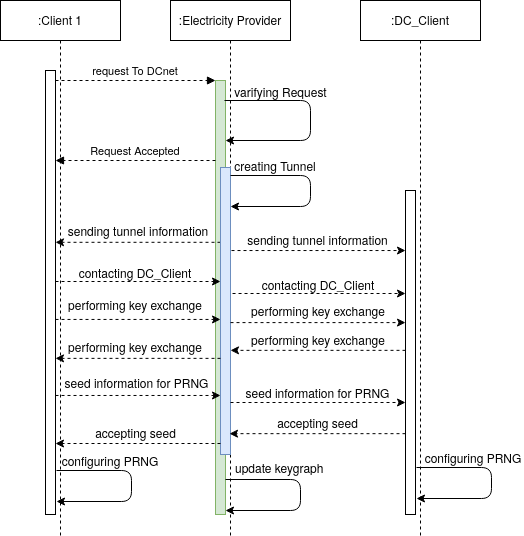
\includegraphics[width=0.8\textwidth]{images/Registering.png}
  \caption[Short description]{An example of a NILM analysis.}
  \label{fig:Appliance_Model}
\end{figure}
An SMGW that wants to register in the DC network sends a special defined request to its power provider. For this purpose the notification field in the header is used and notification 1 is sent. Notification 1 represents a request from the SMGW to register in a DC network. The electricity provider assigns the requesting DC client to a suitable geographical region and suggests a random client (SMGW) which is already registered in the DC network. Afterwards the electricity provider establishes a tunnel and sends the tunnel information to the DC client and the registering client. Via this tunnel it is possible for the two SGMW to create a communication link via the electricity provider. If an SMGW sends to the tunnel, the message is forwarded to the future neighbor. The DC client which is already present in the DC network is only informed by the electricity provider that it receives a new neighbor and has to exchange contact information. The requesting SMGW needs to send the seeds over the tunnel. To prevent the electricity provider from reading the seeds, the clients exchange Diffie Helmann keys via the tunnels provided.%ist das korrekt?
Once the seeds have been exchanged, the power provider is informed by the requesting client that it has successfully entered the DC network by notification 2. The PRNGs generate the keys that are added or subtracted to the message to create the local superposition. The procedure was explained in more detail in ref.%erklärung zu PRNGs
Afterwards all participants in the DC network can send their local superpositions to the power provider. The provider forms the global superposition and receives the aggregated power consumption of all SMGWs in the DC network. If necessary, the electricity supplier must ensure that in the future messages can continue to be exchanged between registered customers via the same tunnel. The already registered clients can therefore not choose which new communication partners they get. In addition it is assumed that the electricity provider has already been authorized by the SWA. Otherwise, the SMGW would not be able to establish a connection to the supplier.\\
%(der Gedanke ist, dass es viele verschiedene kleine DC-Netze gibt, die getrennte Schlüsselgraphen besitzen, jedes DC-Netz sendet seine lokale Summe an den Stromanbieter, der alle Werte aufsummiert und die globale Summe bildet (für ein DC-Netz)
\\
\textbf{SGMW Normal Operation}
\\
\\
%wie sieht eine normale Operation aus? wie häufig wird gesendet? wofür wird das transmisson bit verwendet? und der timestampt
So far, the steps to initialize a DC grid into the already operating power grid have been explained. Next, a description is given of how the technical process takes place in the DC grid, assuming that no faults occur or corrective measures need to be taken. The SMGW transmits its electricity consumption periodically from the moment it enters the DC network. The time period is defined by the electricity provider. For the DC network, it is most practical if all SMGWs send their local superposition to the power supplier at the same time or within a short transmission interval (e.g. one minute). This can be done without problems, because according to ref 3.1 all SMGW must update their time in regular intervals with NTP servers. If an SMGW has not sent a local superposition within the transmission interval, corrective measures are implemented. The frame that a SGMW sends to the power provider is filled in as follows:
\begin{enumerate}
\item DC Net Identifier:\\
The DC net in which the SMGW is registered is entered here.
\item Client Identifier:\\ 
The assigned client identifier is sent in this field.
\item Transmission Bit:\\
This field is exactly 1 bit and is set to 1 when a local superposition is sent.
\item Time Stamp:\\
A time stamp is appended when the frame is generated.
\item Notification:\\
Notification message 5 is sent to inform the electricity provider that this message is a local superposition.
\item Data:\\
Generated local superposition is entered in the data field.
\end{enumerate}
The electricity provider processes the received frames according to the following procedure:\\
\begin{enumerate}
\item DC Network Identifier:\\
DC Network Identifier indicates to which DC net the message is processed.
\item Client Identifier:\\
The Client Id of the frame is stored in a memory structure. In the memory structure can be looked up later, which client has not sent a locale superposition in the round.
\item Transmission Bit: Each message has a transmission bit set to 1. All transmission bits are added up and at the end of the round it can be checked whether all SMGWs have sent their local sum. If the summed transmission bits do not correspond to the number of participants in the DC network, correction procedures must be applied.
\item Time Stamp: The power supplier can assign the message to the correct round.
\item Notfication: Notification message 5 informs the electricity supplier that the local superposition is being transmitted.
\item Data:
The local superposition in the field is added up with all other superpositions and the electricity provider gets the global superposition. This is the aggregated power consumption of all SMGWs in the DC network.
\end{enumerate}
\\
\\
\textbf{SGMW Exit from the DC Network}
\\
\\
\begin{figure}[tbp]
  \centering
  \includegraphics[width=0.8\textwidth]{images/Exit.png}
  \caption[Short description]{An example of a NILM analysis.}
  \label{fig:Appliance_Model}
\end{figure}
An exit can be caused, for example, when the customer changes the electricity provider. Then a defined message is sent to the electricity provider. The electricity provider informs the neighbors of the exiting client with a notification message 3. However, to prevent the notification from being misused by the power supplier, notification 3 can only be sent following the exit of an SMGW. Otherwise, a malicious electricity provider would be able to change the structure of the DC network at will. In addition to the notification message 3, the DC Client Identifier of the exiting SMGW is sent as well. This notification signals to the neighbors of the exiting SMGW that they must discard their PRNG configurations to client X and that they must not be used in the calculation of the local superposition in the next round. In order to avoid a synchronization error in the DC network, the "neighbors" must confirm to the power provider that all seeds have been discarded. Otherwise the case may occur that a SMGW continues to add the old key to its message. This would result in a useless global sum. Furthermore, the key graph must be considered. It could be the case that the underlying key graph splits into two DC networks. If this is the case, two separated DC networks are sending to the same DC network identifier. In the example of Figure 3.3, this could happen if Sabine and Rüdiger throw away their shared key. The result is different depending on the position where a DC net splits. But at least one DC network experiences a significant loss of anonymity due to the smaller number of participants that can be aggregated. In the case of particularly serious splits, it can even lead to a participant being completely disconnected from the DC network. If a disconnected client notices that it no longer has any neighbors, it sends a special emergency message to the power provider. Then a new registration process is initiated before the next round starts.\\ To avoid splitting into two DC networks, the exiting SMGW informs its neighbors with which direct partners it was connected. These then initiate a registration process and exchange keys with each other. The fact that all neighbors have exchanged keys with each other guarantees that a DC network does not split when an SMGW leaves. Furthermore, all participants have to have a minimum number of 3 neighbors. This makes the possibility of disconnection from the DC grid much less likely, since several neighbors would have to leave the DC grid at the same time for a participant to be exposed.\\
\\ 
\textbf{SGMW Connection loss}
\\
\\
SMGWs have an Internet connection with which they can communicate via the WAN. If the Internet connection is interrupted, this can lead to an SMGW not being able to send its local superposition in time. The result is that the electricity provider cannot calculate a meaningful global sum in the round. The electricity provider notices the error immediately because the global transmission bit does not correspond to the number of participants in the DC network. In this case, the following corrective actions are implemented: %vllt noch gliedern in 1. locate errorneous client 2. korrektur via local sum 3. save keys von client 4. restore keygraph when client is back up
The electricity provider detects which SMGW has not sent a local superposition based on the client identifier. Since the SMGW sends a complete header and the client identifier of an SMGW is also sent underneath, an electricity provider only has to check which client identifier was not sent. The missing client identifier is also the client that is defective. Once the defective client is located, notification 4 is sent by the power provider to the neighbors of the defective client. The notification contains the Client Identifier of the defective client and requests the neighbors to recalculate their local superposition, but without using the key of the defective client. Afterwards the local superposition is  resent to the electricity provider. Even though the first attempt failed the electricity provider can calculate a meaningful global sum by using the resent local superposition instead of the old local superposition. At the same time, the keys of the defective client are stored by the neighbors in a backup, so that when the defective client re-enters the DC network, the same key graph is restored. The neighbors of the defective client experience no loss of anonymity during the correction process.%vllt noch schreiben weil jeder client mehr als eine verbindung hat
After this procedure, the defective client is temporarily no longer in the DC network. As soon as the SMGW obtains an Internet connection, it must register again in the DC network. The power consumption of the SMGW during the time of Internet loss is not retransmitted. This is because retransmission the power consumption would lead to a complete loss of anonymity. The electricity provider knows at which time stamp which smart meter was defective and could assign the resent electricity consumption directly. In addition, the electricity provider knows how many smart meters are functional at any time and how many are defective through the transmission bit and the assigned number of subscribers in the DC network. With this information, the electricity provider is able to ensure good network stability without any problems. Especially since the chance of an Internet outage is unlikely. The billing is also done correctly because the billing is calculated on the SMGW. Therefore, the electricity provider does not have to fear any loss of income, even though the electricity consumption is not sent.\\
\\ 
\textbf{Manipulation of the Local Superposition}
\\
\\
\begin{figure}[tbp]
  \centering
  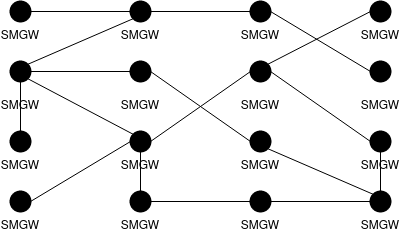
\includegraphics[width=0.5\textwidth]{images/DC Net before Split.png}
  \caption[Short description]{An example of a NILM analysis.}
  \label{fig:Appliance_Model}
\end{figure}
One of the considerations that absolutely must be made in a DC network is: what happens if an SMGW intentionally manipulates the local superposition?
First of all, it must be mentioned that this attack does not help the customer at all to avoid the electricity costs. This is because the electricity costs are calculated by a separate procedure and therefore the billing cannot be affected by the attack. If this problem does occur, it should rather be assumed that it is an external attacker who has taken over an SMGW and wants to sabotage the availability of the DC network.
If the local superposition is manipulated, e.g. by deliberately sending a wrong local superposition, it is no longer possible for the power supplier to calculate a meaningful global superposition. Ergo, it is not possible to see the aggregated power consumption for the whole DC grid. In the case of the attack, the electricity provider cannot assume that the situation will resolve itself and must take measures to find the manipulating SMGW. Furthermore, it must be assumed that the attacker is well aware that the electricity provider will be looking for him. Therefore, the procedure must be designed in such a way that the attacker is found even though he tries to conceal his identity.
For this purpose, a slightly modified version of Prof. Dr Pfitzmann's error localization and recovery protocol can be applied. The protocol of Prof. Dr Pfitzmann talks about 2 different modes, the anonymity mode (A-Mode), in which the DC net works normally and the fault tolerance mode (F-Mode), in which defective stations are searched for.
The F-mode can be extended in this application so that an attacker can also be searched for. If there is an incorrect calculation in the global sum, this is communicated publicly by the power supplier to the SMGW. All SMGWs then save the keys from the last round. The power provider saves all receiving local sums from the round and enjoys special rights that only prevail in F-mode. In the following, the property of DC networks is exploited that allows a DC network with one meaningful global sum to separate into two DC networks with two separate meaningful global sums.
The algorithm is executed as follows:
1. halve the key graph. 
The power provider has the overview of the key graph and can therefore separate the key graph into two parts. Splitting the graph into two halves should be trivial since the planar separator theorem holds.
If a SMGW is exactly on the border of the bisected key graph and has a neighbor in the other half of the key graph, then this SMGW is informed as a special node by the power provider that the neighbor's key is thrown away for this computation. The temporary throwing away of the keys leads to the splitting of the key graph at that point. The power provider can request an SMGW to throw away a key only in F-mode! All SMGWs in one half of the key graph now retransmit the local sum from the last failed round. The adjacent SMGWs that threw away a key calculate the new correct local sum without the neighbor in the other part of the key graph. This results in all nodes sending the same message from the last round except the special nodes. This allows two global sum to be calculated. One global sum from the first half and one global sum from the second half. So the old DC net round is repeated, but in a split net to reduce the number of possible attacker SMGW. The electricity provider can check by the stored local sum if the same local sum would really be resent and can check the correctness. 
If the formation of a global sum fails in the first half of the dc network, then the attacker is located in the first half and the same procedure is repeated in the first half. If the formation of a global sum fails in the second half of the dc network, then the attacker is located in the second half and the procedure is repeated in the second half. 
If the global sum fails in both halves or is calculated correctly, then the attacker is among the special nodes.
The procedure is continued recursively until it is reduced to one SMGW that is eligible to be the attacker. 

There can be the special case that the attacker SMGW is a special node. Since the special nodes send a recalculated local sum, the power provider cannot immediately rule out whether the attacker is among the special nodes. Therefore, for each bisection, an additional subgraph must be formed in which the former special nodes have no neighbors outside the subgraph. In this way it is possible for the electricity provider to control the local sum when resending the local sum of the former special nodes.
\begin{figure}[tbp]
  \centering
  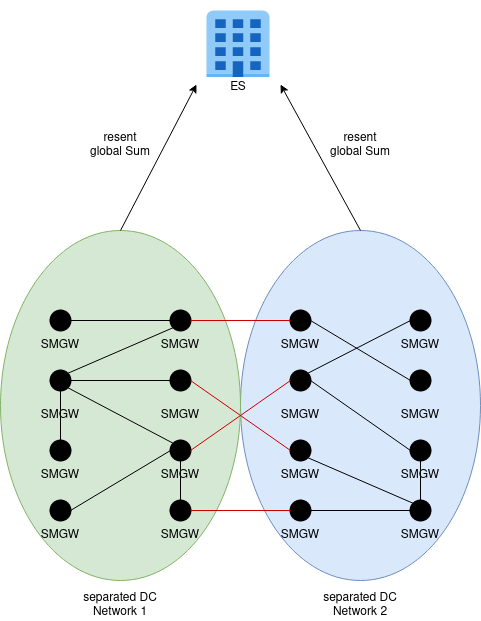
\includegraphics[width=0.5\textwidth]{images/DC Net Split.png}
  \caption[Short description]{An example of a NILM analysis.}
  \label{fig:Appliance_Model}
\end{figure}
%was passiert mit den Sonderknoten? wie wird mit den 3 kanten umgegangen, aber man hat ja am ende nur 2 smgw?
%lsg größere gruppe mit der der angreifer identifiziert wird.
%also wenn nur noch 2 in frage kommen, werden diese beiden in eine größere gruppe gesteckt und geschaut, ob die größere gruppe falsch ist.
\\
\\
\textbf{DC Network Size}
\\
\\
With a small number of participants, conclusions can be drawn about individual participants from the aggregated result. This is the case, for example, if the electricity consumption of one user is equal in percentage to the residual consumption of the other users. Or it is also feasible that a user does not consume any electricity. In a DC network with 2 users, the power consumption would be directly readable even if the individual loads are aggregated. The goal is not to avoid the disclosure of information, but rather to make it hard to draw inferences about an individual user from the aggregated consumption.%quelle
In this thesis, the experiments chapter determines the minimum size of a DC grid to guarantee that statistical inferences are difficult to realize.
On the other hand, it is in the interest of the power supplier not to realize huge DC networks. The more participants a DC network has, the more frequently errors occur that have to be corrected by corrective measures. Although the DC network should scale with many participants, the question arises as to how meaningful the results are when hundreds of participants partially fail.%Etwas über die Größe schreiben, dass die DC netze nicht zu klein sein dürfen, aber es auch vorteile bringt, wenn sie nicht zu groß sind.
\\
\\ 
\textbf{Anonymity}
\\
\\
By using PRNG, anonymity decreases from information-theoretically secure to complexity-theoretically secure anonymity. Nevertheless even if an SMGW is controlled by an attacker, it would not be possible for the attacker to read the power consumption of other SMGWs. This is because the attacker has no access to the global total. This can only be calculated by the electricity provider. With the proposed method, the attacker lacks the necessary information to launch a potential attack on the DC network (if the attacker only has control over one SMGW). Furthermore, the attacker also has no information about the key graph. This further complicates the chances of a successful attack to deanonymize the electricity consumption of costumers. The electricity provider is potentially the most dangerous attacker in the protocol, since the SMGWs cannot communicate with each other, they rely on the electricity provider to register in the DC network. As a result, the power provider has to take over administrative tasks and therefore possesses a lot of control. To ensure that the electricity supplier is not too powerful, its competences have been restricted. The best chance of the electricity provider to break the anonymity to its customers is that the administrative powers are abused to connect individual SMGWs to malicious neighbors. Once the electricity provider manages to link an SMGW with only malicious neighbors, the local sum can be reconstructed and the electricity consumption is visible. This is prevented by forcing the electricity provider to select a random neighbor upon entry and not being able to remove SMGWs from the network on its own. These measures make it almost impossible for the electricity provider to affect the selection of neighbors in the DC network.
%vllt noch schreiben wie das in die technische Richtlinie implementiert werden könnte?


%noch unbedingt schreiben, dass in dem Protokoll unbedingt gewollt ist, dass es zu kollisionen kommt und das in einem normalen DC netz kollisionsauflösungsverfahren angewendet werden. siehe überlagerndes empfangen
\clearpage

%%% Local Variables:
%%% TeX-master: "diplom"
%%% End:
